\subsection{Bicopter}

\begin{figure}[ht]
 \centering
% \def\svgwidth{.5\textwidth}
 \input{graphics/MechModelBicopter.pdf_tex}
 \caption{Model of a bicopter (background image: \url{www.poppaper.net/80155164809})}
 \label{fig:BicopterModel}
\end{figure}

\paragraph{Equations of motion.}
The bicopter considered here is a single rigid body with two tiltable propellers as illustrated in \autoref{fig:QuadModel}.
With the same coordinates as for the previous examples, the equations of motion are identical as well up to the generalized force from the propellers 
\begin{align}
 \genForceInput
 =
 \underbrace{\begin{bmatrix}
  1 & 0 & 1 & 0 \\
  0 & \sin\PropInc & 0 & -\sin\PropInc \\
  0 & \cos\PropInc & 0 & \cos\PropInc \\
  0 & \PropPosY' & 0 & -\PropPosY' \\
  \PropPosZ & 0 & \PropPosZ & 0 \\
  -\PropPosY & 0 & \PropPosY & 0 \\
 \end{bmatrix}}_{\sysInputMat}
 \underbrace{\begin{bmatrix} \PropForce[1] \sin\PropTilt[1] \\ \PropForce[1] \cos\PropTilt[1] \\ \PropForce[2] \sin\PropTilt[2] \\ \PropForce[2] \cos\PropTilt[2] \end{bmatrix}}_{\sysInput}
 .
\end{align}
with $\PropPosY' = \PropPosY \cos\PropInc - \PropPosZ \sin\PropInc$.
The transformation of the actual control inputs $\PropForce[1]$, $\PropForce[2]$ and $\PropTilt[1]$, $\PropTilt[2]$ to a auxiliary input $\sysInput$ is used to achieve the linear form $\genForceInput = \sysInputMat\sysInput$.
Within the input constraints $2\,\unit{N} \leq \PropForce[i] \leq 14\,\unit{N}$, $-30^\circ \leq \PropTilt[i] \leq 30^\circ$, $i=1,2$ this transformation is bijective.
To account for the original constraints in the transformed input $\sysInput\in \RealNum^4$, a convex approximation illustrated in \autoref{fig:BicopterInputConstraintApprox} is used.
These constraints can be written in the required form $\sysInputConstMat \sysInput \leq \sysInputConstVec$.

\begin{figure}[ht]
 \centering
 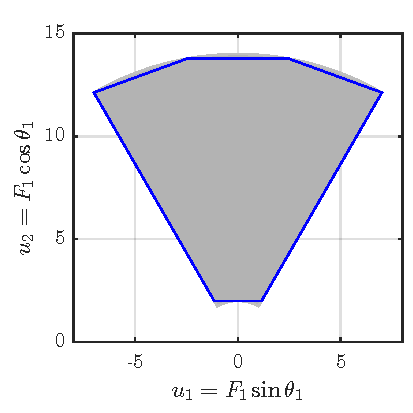
\includegraphics[]{Bicopter/BicopterInputConstraintApprox.pdf}
 \caption{Approximation of the Bicopter input constraints}
 \label{fig:BicopterInputConstraintApprox}
\end{figure}

\paragraph{Reference trajectory.}
A possible left complement for $\sysInputMat$ is
\begin{align}
 (\sysInputMatLComp)^\top = \begin{bmatrix} \PropPosZ & 0 & 0 & 0 & -1 & 0 \\ 0 & \PropPosY' & 0 & -\sin\PropInc & 0 & 0 \end{bmatrix}
\end{align}
With this, the matching condition for the reference from \eqref{eq:MatchingForceZeroError} is
\begin{align}
 \tuple{\lambda}^{\text{ZeroError}} = 
% \begin{bmatrix} 
%  m \PropPosZ (\vxd + \vy\wz \!-\! \vz\wy + \Rzx\gravityAccConst ) - (\Jy\wyd + (\Jx-\Jz)\wx\wz)  \\
%  \PropPosY' m (\vyd + \vx\wz \!-\! \vz\wx + \Rzy\gravityAccConst) - \sin\PropInc (\Jx \wxd + (\Jz-\Jy)\wy\wz)
% \end{bmatrix}
 \begin{bmatrix} 
  m \PropPosZ  \big( \vxd + \vy\wz \!-\! \vz\wy - \epsx (\wyd + \tfrac{\Jx-\Jz}{\Jy} \wx\wz) + \Rzx\gravityAccConst \big)  \\
  m \PropPosY' \big( \vyd + \vx\wz \!-\! \vz\wx + \epsy (\wxd + \tfrac{\Jz-\Jy}{\Jx} \wy\wz) + \Rzy\gravityAccConst \big)
 \end{bmatrix}
 = \tuple{0}
 .
\end{align}
where
\begin{align}
 \epsx = -\tfrac{\Jy}{\m \PropPosZ},
\qquad
 \epsy = \tfrac{\Jx \sin\PropInc}{\m (\PropPosY \cos\PropInc - \PropPosZ \sin\PropInc)}.
\end{align}
For the general case\footnote{Even in the case $\epsx=\epsy\neq0$ we would need $\Jx=\Jy=\Jz$ for $\r+\R \tuple{\eps}$ to be a flat output. The case $\epsx=0$ implies $\Jy=0$, which does not make physical sense.} 
$\epsx\neq\epsy$ this system is probably not flat, so parameterization of a feasible reference trajectory is not trivial.

\paragraph{Closed loop template.}
As for the quadcopter, the closed loop templates are that of a free rigid body i.e.\ \autoref{sec:CtrlApproachParticlesSingleBody}, \autoref{sec:CtrlApproachBodySingleBody} and \autoref{sec:CtrlApproachEnergySingleBody}.
However, in contrast to the quadcopter there are no assumptions on symmetries in the constitutive parameters.

\paragraph{Matching.}
As before we first consider the linearized matching conditions:
It turns out that asymmetries in the constitutive parameters are not useful for resolving matching constraints.
So we set $\Jcxy=\Jcxz=\Jcyz=0$, $\scx=\scy=0$ and the same for damping and stiffness.
The remaining linearized matching conditions may be fulfilled by constraining the parameters as
\begin{subequations}
\begin{align} 
 \lcz = \hcz,
\qquad
 \sigcx = \sigcy = 0,
\qquad
 \kapcx = \kapcy = \mc \gravityAccConst (\hcz-\scz),
\\
 \Jcx = \mc (\hcz-\scz)(\scz-\epsy),
\qquad
 \Jcy = \mc(\hcz-\scz) (\scz-\epsx),
\end{align}
\end{subequations}
which leaves the tuning parameters $\mc, \dc, \kc, \scz, \hcz$ and $\Jcz, \sigcz, \kapcz$.
Note, in contrast to the quadcopter, that $\epsx \neq \epsy$ implies $\Jcx \neq \Jcy$ and since the remaining relevant parameters are identical, the closed loop dynamics for x and y are different from another.

The remaining matching force in the stabilization case $\sysVelR = \tuple{0}$ is
\begin{align}
 \tilde{\sysForce} = \frac{\mc}{m}
 \begin{bmatrix} \frac{1}{\hcz-\epsx} & 0 \\ 0 & \frac{1}{\hcz-\epsy} \\ 0 & 0 \\ 0 & -\frac{\epsy}{\hcz-\epsy} \\ \frac{\epsx}{\hcz-\epsx} & 0 \\ 0 & 0 \end{bmatrix}
 \begin{bmatrix}
  \big( \Jcz - \mc(\hcz-\scz) (\tfrac{\Jx-\Jz}{\Jy}\epsx - \epsy) \big) \wy\wz - \tfrac{1}{2} \kapcz (\RExz+\REzx) \\
  \big( \Jcz - \mc(\hcz-\scz) (\tfrac{\Jy-\Jz}{\Jx}\epsy - \epsx) \big) \wx\wz - \tfrac{1}{2} \kapcz (\REyz+\REzy)
 \end{bmatrix}
\end{align}

\paragraph{Simulation result.}
Since the bicopter model is probably not flat, generation of a feasible reference trajectory is not trivial. 
For the simulation example here we exploited that, if we set $\rRx = 0$ and $\RRxx=1$, the motion is constrained to the yz plane and the remaining model is essentially a PVTOL.
The reference trajectory chosen for this example is a vertical circle with constant arc speed in the yz plane, similar to the examples presented in \cite{Konz:AT} and \cite{Konz:GaussTrackingControl}.
As shown in \autoref{sec:CtrlExamplePVTOL}, the position trajectory determines the tilt trajectory through flatness.
The circle arc speed was chosen such that the bicopter is upside down at the highest point of the circle.

As initial condition for the simulation we chose a position error of $0.5\,\unit{m}$ in all directions and heading error of $90^\circ$. 
This guarantees that all parts of the control are exited.

\begin{figure}[t]
 \centering
 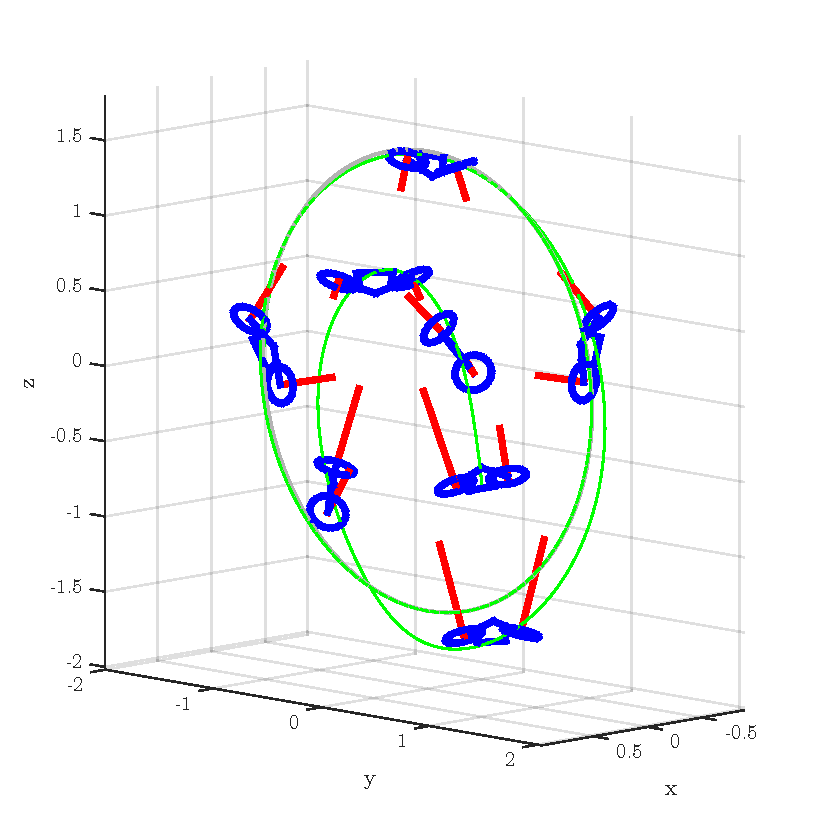
\includegraphics[]{Bicopter/BicopterCircleSimSnapshots.pdf}
 \caption{Snapshots for the simulation of the bicopter}
 \label{fig:BicopterCircleSimSnapshots}
\end{figure}

The simulation result for the position trajectory with snapshots of a bicopter mockup for the first $3\,\unit{s}$ is shown in \autoref{fig:BicopterCircleSimSnapshots}.
The red lines indicate the propeller tilt and the thrust magnitude.
The resulting time graphs are shown in \autoref{fig:BicopterCircleSimRes}.
Roughly, during the first loop, or the first $2\,\unit{s}$, the state trajectory converges to its reference and tracks it for the remaining simulation time.
This is also quantified by the error energy $\totalEnergyC$ in the bottom of \autoref{fig:BicopterCircleSimRes}.
There, one may also see that $\totalEnergyCd \neq \accCtrl{\mathcal{P}}$ which is most notably during the time around $t=0.5\,\unit{s}$ when input constraints are active, but also due to the non-vanishing matching force $\tilde{\sysForce}$.
Nevertheless, if we neglect the parts where the input constraints are active, the error energy is converging to zero.
So, even for this arguably challenging example, the control objective is achieved.

\begin{figure}[p]
 \centering
 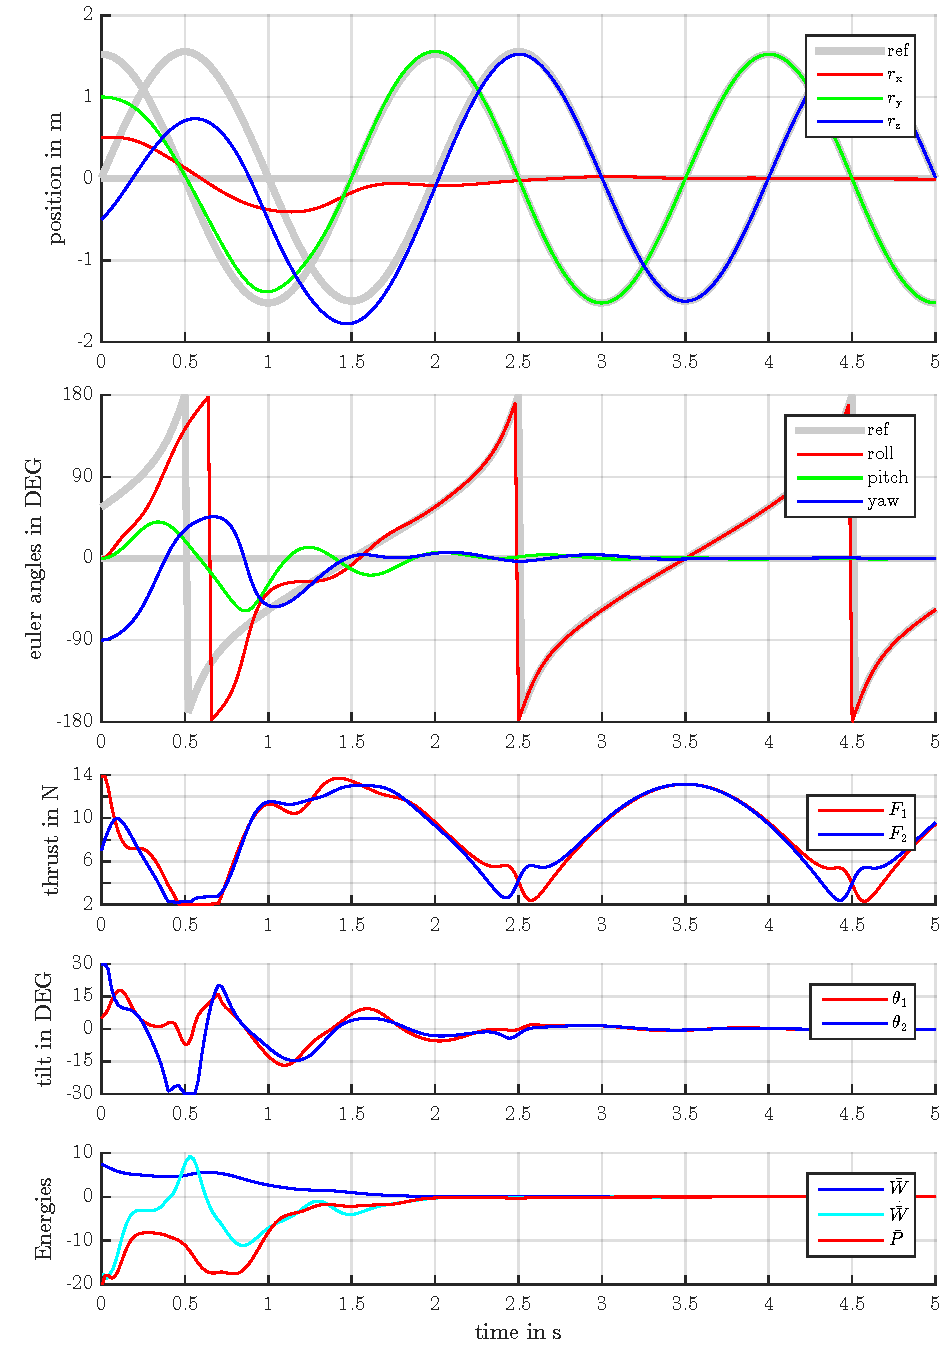
\includegraphics[]{Bicopter/BicopterCircleSimRes.pdf}
 \caption{Simulation result for the bicopter}
 \label{fig:BicopterCircleSimRes}
\end{figure}
